% --- RAG evaluation ---
\begin{frame}{Evaluating RAG Means Evaluating Two Systems}
  \begin{columns}[T,onlytextwidth]
    \column{0.5\textwidth}
      \begin{itemize}\footnotesize\itemsep0.32em
        \item[\textcolor{red}{$\blacktriangleright$}] A retrieval-augmented pipeline has two failure surfaces, and an end-to-end score cannot tell them apart. ``The answer was wrong'' is not an actionable finding.
        \item[\textcolor{red}{$\blacktriangleright$}] \textbf{Retrieval failure:} the evidence needed was never fetched. No amount of generator improvement fixes this --- the information is not in the context.
        \item[\textcolor{red}{$\blacktriangleright$}] \textbf{Generation failure:} the evidence \textit{was} in the context and the model still hallucinated, contradicted it, ignored it, or answered a different question.
        \item[\textcolor{red}{$\blacktriangleright$}] So a RAG evaluation reports at least three things: \textbf{did we retrieve the right context}, \textbf{is the answer grounded in the context we did retrieve}, and \textbf{does the answer address the question}.
        \item[\textcolor{red}{$\blacktriangleright$}] Note the middle one is deliberately independent of correctness. An answer faithful to a wrong document is a \textit{retrieval} bug; scoring it as a generation bug sends you to fix the wrong component.
      \end{itemize}
    \column{0.48\textwidth}
      \centering
      \vspace{0.6em}
      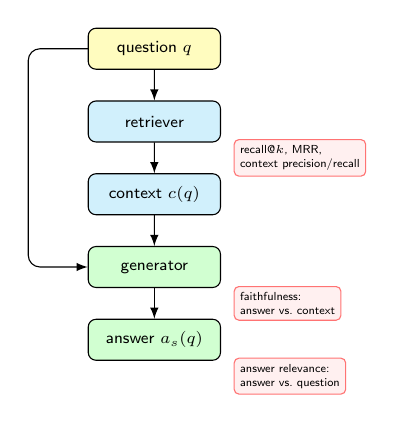
\begin{tikzpicture}[font=\sffamily\scriptsize, >=latex, scale=0.84,
          every node/.style={transform shape},
          box/.style={draw, rounded corners=0.1cm, align=center, minimum width=2.0cm, minimum height=0.62cm},
          q/.style={box, fill=yellow!25},
          r/.style={box, fill=cyan!18},
          g/.style={box, fill=green!18},
          mlab/.style={font=\sffamily\tiny, align=left, anchor=west, draw=red!55,
                       fill=red!6, rounded corners=0.06cm, inner sep=2.5pt}]
        \node[q] (query) at (0,3.2) {question $q$};
        \node[r] (ret)   at (0,2.1) {retriever};
        \node[r] (ctx)   at (0,1.0) {context $c(q)$};
        \node[g] (gen)   at (0,-0.1) {generator};
        \node[g] (ans)   at (0,-1.2) {answer $a_s(q)$};
        \draw[->] (query) -- (ret);
        \draw[->] (ret)   -- (ctx);
        \draw[->] (ctx)   -- (gen);
        \draw[->] (gen)   -- (ans);
        % the question also conditions the generator directly
        \draw[->, rounded corners=0.15cm] (query.west) -- ++(-0.9,0) |- (gen.west);
        \node[mlab] at (1.2,1.55)  {recall@$k$, MRR,\\context precision/recall};
        \node[mlab] at (1.2,-0.65) {faithfulness:\\answer vs.\ context};
        \node[mlab] at (1.2,-1.75) {answer relevance:\\answer vs.\ question};
      \end{tikzpicture}\\[0.3em]
      {\scriptsize Each metric attaches to one edge of the pipeline, so a failing metric names the component to fix.}
  \end{columns}
\end{frame}

\begin{frame}{Retrieval Metrics}
  \begin{itemize}\footnotesize\itemsep0.05em
    \item[\textcolor{red}{$\blacktriangleright$}] Let $R_q$ be the set of relevant items for query $q$ and $T_k(q)$ the top-$k$ retrieved items.
    \item[\textcolor{red}{$\blacktriangleright$}] \textbf{Recall@$k$} --- did we fetch the evidence at all? This is the ceiling on everything downstream:
      \[ \text{Recall@}k = \frac{|R_q \cap T_k(q)|}{|R_q|}, \qquad \text{Precision@}k = \frac{|R_q \cap T_k(q)|}{k}. \]
    \item[\textcolor{red}{$\blacktriangleright$}] \textbf{Mean reciprocal rank} --- how high did the \textit{first} relevant item land? Appropriate when one good document suffices:
      \[ \text{MRR} = \frac{1}{|Q|}\sum_{q \in Q} \frac{1}{\text{rank}_q}, \]
      contributing $0$ when nothing relevant was retrieved.
    \item[\textcolor{red}{$\blacktriangleright$}] \textbf{nDCG@$k$} --- graded relevance with a position discount, normalised by the ideal ranking:
      \[ \text{nDCG@}k = \frac{\text{DCG@}k}{\text{IDCG@}k}, \qquad \text{DCG@}k = \sum_{i=1}^{k} \frac{2^{\text{rel}_i} - 1}{\log_2(i+1)}. \]
      The linear-gain form $\sum \text{rel}_i / \log_2(i+1)$ is also standard --- \textbf{state which you used}, since they differ for graded relevance.
    \item[\textcolor{red}{$\blacktriangleright$}] For RAG specifically, \textbf{recall@$k$ matters more than precision@$k$}: a long-context generator tolerates some irrelevant passages, but cannot invent a passage that was never fetched. Measure recall at the $k$ you actually pass to the model.
  \end{itemize}
\end{frame}

\begin{frame}[allowframebreaks]{RAGAS: Reference-Free Metrics for RAG}
  \begin{itemize}\footnotesize\itemsep0.3em
    \item[\textcolor{red}{$\blacktriangleright$}] The point of RAGAS is \textbf{reference-free} evaluation: it needs the question, the retrieved context, and the answer --- but no gold answer. That is what makes it usable on production traffic.
    \item[\textcolor{red}{$\blacktriangleright$}] The paper defines exactly \textbf{three} metrics, each computed by prompting an LLM to decompose the text and then counting:
      \begin{itemize}\itemsep0.25em
        \item \textbf{Faithfulness.} Extract the set $S$ of statements made by the answer; verify each against the context $c(q)$; let $V \subseteq S$ be those that can be inferred from it. Then
          \[ F = \frac{|V|}{|S|}. \]
          This is the hallucination metric: it asks whether the answer is \textit{supported}, regardless of whether it is true.
        \item \textbf{Answer relevance.} Reverse-generate $n$ questions $q_1,\dots,q_n$ \textit{from the answer}, embed them, and compare to the original question:
          \[ \text{AR} = \frac{1}{n}\sum_{i=1}^{n} \operatorname{sim}(q, q_i). \]
          An answer that rambles or dodges produces questions unlike the one asked.
        \item \textbf{Context relevance.} Have the LLM extract the sentences of the context that are essential to answering, and take
          \[ \text{CR} = \frac{|\text{extracted sentences}|}{|\text{sentences in } c(q)|}. \]
          Low values mean the retriever is padding the context with noise.
      \end{itemize}
    \item[\textcolor{red}{$\blacktriangleright$}] Validated on \textbf{WikiEval}, 50 question--context--answer instances built from 50 Wikipedia pages edited after the start of 2022, annotated by two humans (agreement about 95\% on faithfulness and context relevance, 90\% on answer relevance).
  \end{itemize}
  \vspace{0.1em}
  {\scriptsize Es, James, Espinosa-Anke, Schockaert, ``RAGAs: Automated Evaluation of Retrieval Augmented Generation,'' EACL 2024 System Demonstrations, \href{https://arxiv.org/abs/2309.15217v2}{arXiv:2309.15217v2}.}
\end{frame}

\begin{frame}[allowframebreaks]{The Library Has Moved On From the Paper}
  \begin{itemize}\footnotesize\itemsep0.3em
    \item[\textcolor{red}{$\blacktriangleright$}] A trap worth naming explicitly: the metric \textit{names} in today's \texttt{ragas} library no longer mean what the paper's names mean. Do not present them as the same objects.
      \begin{itemize}\itemsep0.15em
        \item The paper's \textbf{answer relevance} is now called \textbf{response relevancy}.
        \item The paper's \textbf{context relevance} (the sentence ratio) is gone; the library's current \textbf{context relevance} is a different, Nvidia-contributed metric.
        \item \textbf{Answer correctness} has been split into \textbf{factual correctness} and \textbf{semantic similarity}.
      \end{itemize}
    \item[\textcolor{red}{$\blacktriangleright$}] The two retrieval metrics you will actually use are reference-based:
      \[ \text{Context Precision@}K = \frac{\sum_{k=1}^{K} \left(\text{Precision@}k \times v_k\right)}{\text{number of relevant items in the top } K}, \quad v_k \in \{0,1\}, \]
      which rewards ranking relevant chunks \textit{high}, not merely retrieving them; and
      \[ \text{Context Recall} = \frac{\text{claims in the reference answer supported by the retrieved context}}{\text{total claims in the reference answer}}, \]
      which asks whether the context contained everything the ideal answer needed.
    \item[\textcolor{red}{$\blacktriangleright$}] Other metrics in the current set worth knowing: \textbf{context entities recall} (did we retrieve the named entities the answer needs?) and \textbf{noise sensitivity} (does adding irrelevant context degrade the answer?).
    \item[\textcolor{red}{$\blacktriangleright$}] \textbf{Pin the library version} in your report. A metric whose definition changed between releases is not a time series.
  \end{itemize}
  \vspace{0.1em}
  {\scriptsize Metric definitions from the RAGAS documentation, \href{https://docs.ragas.io/en/stable/concepts/metrics/available_metrics/}{docs.ragas.io}.}
\end{frame}

\begin{frame}[allowframebreaks]{Grounding, Citations, and Stronger RAG Evaluators}
  \begin{itemize}\footnotesize\itemsep0.3em
    \item[\textcolor{red}{$\blacktriangleright$}] \textbf{Citation checks} are the cheapest grounding signal and belong in every RAG system, judge or no judge:
      \begin{itemize}\itemsep0.12em
        \item \textbf{Citation validity} --- does every cited identifier exist in the retrieved set? A pure string check; a failure is a hallucinated source.
        \item \textbf{Citation support} --- does the cited passage actually entail the sentence it is attached to? Check with a natural-language-inference model or a judge.
        \item \textbf{Coverage} --- what fraction of the answer's factual sentences carry any citation at all?
      \end{itemize}
    \item[\textcolor{red}{$\blacktriangleright$}] A small fine-tuned \textbf{NLI model} is often a better entailment checker than a large general judge: cheaper, deterministic, and trained for exactly this decision.
    \item[\textcolor{red}{$\blacktriangleright$}] \textbf{ARES} takes the trained-judge idea further: generate synthetic training data, fine-tune lightweight judges for context relevance, answer faithfulness, and answer relevance, then \textbf{correct the judges' residual error} using a few hundred human annotations via prediction-powered inference --- which also yields confidence intervals on the result.
    \item[\textcolor{red}{$\blacktriangleright$}] \textbf{RAGChecker} attacks the attribution problem: claim-level diagnostics that assign each error to the retriever or the generator, so the metric tells you which team owns the bug.
    \item[\textcolor{red}{$\blacktriangleright$}] \textbf{Whatever you use, build a small gold set for your own corpus.} Twenty to fifty questions with hand-marked relevant passages will teach you more about your retriever than any off-the-shelf metric.
  \end{itemize}
  \vspace{0.1em}
  {\scriptsize Saad-Falcon, Khattab, Potts, Zaharia, ``ARES,'' NAACL 2024, \href{https://arxiv.org/abs/2311.09476v2}{arXiv:2311.09476v2}; Ru et al., ``RAGChecker,'' \href{https://arxiv.org/abs/2408.08067v2}{arXiv:2408.08067v2}.}
\end{frame}
